\chapter{Computational Study}\label{chapter:study}
This chapter tests \gls{drispi} on the 100 XL instances of Queiroga et al.\ (2026)
against the eight monolithic solvers benchmarked there. The study aims to answer two questions:
The first is whether an adaptive decomposition framework that learns its
decomposition and routing choices during a run can match state-of-the-art
monolithic solvers at this scale. The second is whether the weights HAOS learns along the way provide interpretable 
insights about the instances they were learned on.

Section~\ref{sec:stu-experiment} describes the dataset, specifies implementation and
hardware specificiations, the parameter values, and explains expertimental design choices. Section~\ref{sec:stu-results} shows and analyzes the results. Here we answer the primary and secondary research questions through comparison with the published solvers, breaks the results down by instance characteristics, and examines the learned HAOS weights and the convergence of
individual runs.

\section{Experimental Design}\label{sec:stu-experiment}
All 100 instances are solved by the same \gls{drispi} configuration. Nothing is tuned
per instance by design without anyexceptions. Section~\ref{sec:stu-dataset} describes the instances and the reference solutions used as baseline, section~\ref{sec:stu-implementation} the software and hardware the campaign
ran on, section~\ref{sec:stu-hyperparameters} the parameter values, and
section~\ref{sec:stu-repetitions} the number of seeds and the statistical precision it buys for our experiment.

\subsection{Dataset}\label{sec:stu-dataset}
The XL set (section~\ref{sec:lit-problem}) extends the generation scheme of the X
instances of \citet{uchoaNewBenchmarkInstances2017} to up to 10,000 customers. Every instance
places its nodes on a $[0, 1000] \times [0, 1000]$ grid with Euclidean distances
and combines one level of each of four attributes. The depot is Random, Central
at $(500, 500)$, or Eccentric at $(0, 0)$ in the bottom left corner. Customers are Random, Clustered, or
Random-Clustered around a small number of seed points. Demand follows one of
seven distributions: unitary (U), four ranges of increasing width (1--10, 5--10,
1--100, 50--100), a quadrant-dependent range (Q), or many small and few large
demands (SL). The target average route length $r$ lies in one of seven bands,
from ultra-short ($r \in [3, 5]$) to ultra-long ($r \in [50, 200]$), and
capacity $Q$ is set so that a solution with the minimum number of routes attains
it. The instance name references $n$ and that minimum route count, e.g.\
XL-n4535-k1134. This $k$ equals $\lceil \sum_{i=1}^{n} q_i / Q \rceil$, making it the mathematical minimum number of routes, because fewer vehicles could not carry the total customer demand under capacity set to $Q$. This $k$ is
fixed by the benchmark and unrelated to the subcluster count $k$ of Section~\ref{sec:fra-haos}.
Table~\ref{tab:xl-summary} breaks down the above mentioned characteristics on a per-instance basis along with \gls{drispi}'s result and comparison to initial and current \gls{bks} values.

The initial BKS values of \citet{queirogaXLInstancesCapacitated2026} come from the solver
runs described in section~\ref{sec:lit-large-cvrp} and were released as baselines with the
CVRPLib BKS Challenge, a community competition opened on January~12, 2026, in
which any team can submit an improved solution for automatic verification. By
the current record,\footnote{\url{https://galgos.inf.puc-rio.br/cvrplib/index.php/en/bks_challenge/score/instances}, accessed September 7, 2026.} the challenge has improved 99 of the 100
initial values, leaving only XL-n1094-k157 to still hold its initial value. We report the
percentage gap to baselines such as the initial and the current \gls{bks}:
\begin{equation}
\mathrm{Gap} = 100 \times \frac{c - c_{\mathrm{BKS}}}{c_{\mathrm{BKS}}}.
\label{eq:gap}
\end{equation}
The quantity $c$ is the reported solution cost. The current
\gls{bks} represents the official best known solution. However, we primarily compare against initial \gls{bks}, because published solvers produced it in two-hour single-thread runs on specified hardware
(Section~\ref{sec:lit-large-cvrp}), using us an experimental design we can reproduce to allow for any algorithmic comparability. The official BKS values on the other hand have been achieved without constraints regarding computational, with many of them coming from day-long runs that rely on raw compute, rendering any fair comparison infeasible.

\subsection{Framework Implementation}\label{sec:stu-implementation}
All experiments in this chapter run on a single, shared department server under
Ubuntu 22.04.5 LTS with two Intel Xeon Platinum~8280L CPUs at 2.70\,GHz
(28 cores each, 56 cores and 112 threads total) and 5,928\,GiB of RAM, with no
GPU\@. \gls{drispi} runs inside Docker containers (Docker 28.1.1) pinned to a disjoint physical-core range with \texttt{--cpuset-cpus}. This pinned CPU count, not a library thread-pool default, sets the framework's parallelism budget.

The campaign presented in section~\ref{sec:stu-comparison} is comprised of all 100 instances, each run on three seeds with a wallclock runtime budget and termination criterion of T=2h (300 runs, 7{,}200 seconds each). For that we pin 48 of the server's 56 physical cores as six exclusive 8-core Docker containers, three per socket, parallelizing as outlined in section~\ref{sec:fra-pipeline} with a split into six DRI workers, one BG-AILS worker, and one SP worker. SMT siblings are left idle. Runs are packed into waves ordered by instance size so that the three seeds of the largest instance, XL-n10001-k1570, never share a wave. The full campaign takes 50 waves and about 100 hours of wall-clock time.

\gls{drispi} uses Python 3.11, with dependencies locked via \texttt{uv}: Libraries PyVRP 0.13.3 (HGS-CVRP), scikit-learn 1.8.0 (K-Means and Agglomerative Clustering), scikit-learn-extra 0.3.0 (K-Medoids), scikit-fuzzy 0.5.0 (Fuzzy C-Means), gurobipy 13.0.1 (SC/SP), and vrplib 2.1.0 for instance parsing. AILS-II, FILO, and FILO2 are vendored as git submodules pinned to a fixed commit each and compiled at image build time, rather than resolved from a floating branch, so a rebuild reproduces the exact binaries behind the results in Section~\ref{sec:stu-comparison}. The whole framework runs inside a Docker image built from this locked environment, so the software stack behind every reported run is fixed independently of the host it executes on.

\subsection{Hyperparameters}\label{sec:stu-hyperparameters}
\begin{table}[!htb]
\centering\small
\caption{Hyperparameters of the Benchmark Configuration.}
\label{tab:hyperparameters}
\begin{tabular}{@{}lll@{}}
\toprule
Parameter & Value & Defined in \\
\midrule
\multicolumn{3}{@{}l}{\emph{HAOS}} \\
Warm-up iterations & 10 & Section~\ref{sec:fra-haos} \\
Decay $\gamma$ & 0.95 & Equation~\ref{eq:haos-decay} \\
Starting weight $w_0$ & 10.0 & Equation~\ref{eq:haos-update} \\
Floor $p_{\min}$: $k$ / $\lambda_q$, method, solver / paradigm & 0.025 / 0.05 / 0.10 & Equation~\ref{eq:haos-probability} \\
Immediate and deferred rewards & Table~\ref{tab:haos-rewards} & Section~\ref{sec:fra-haos} \\
\addlinespace
\multicolumn{3}{@{}l}{\emph{Decomposition and routing}} \\
Base $k$ arms & $\{2,3,4,6,8,10,12\}$ & Section~\ref{sec:fra-haos} \\
Maximum number of $k$ arms & 10 & Section~\ref{sec:fra-haos} \\
Minimum routes per subcluster & 8 & Section~\ref{sec:fra-haos} \\
Minimum spacing between $k$ arms & 2 & Section~\ref{sec:fra-haos} \\
Subcluster time budget & $\max(5\,\mathrm{s},\ 0.06\,\mathrm{s} \cdot n_c)$ & Section~\ref{sec:fra-routing} \\
\addlinespace
\multicolumn{3}{@{}l}{\emph{BG-AILS}} \\
Boundary threshold $\tau$ & 0.5 & Equation~\ref{eq:bg-ails-threshold} \\
Small-cluster cap $\sigma$ / boost $\alpha$ & 20 / 0.5 & Equation~\ref{eq:bg-ails-weighted} \\
Initial $\omega_0$ & 10 & Section~\ref{sec:fra-bg-ails} \\
First-route selection & greedy, unique first & Section~\ref{sec:fra-bg-ails} \\
Chain length & $k$ & Section~\ref{sec:fra-bg-ails} \\
Boundary mask on first local search & on & Section~\ref{sec:fra-bg-ails} \\
Budget floor / margin & 60\,s / 1.0 & Equation~\ref{eq:bg-ails-budget} \\
\addlinespace
\multicolumn{3}{@{}l}{\emph{Route pool, SC/SP, and improvement}} \\
Maximum pool size & 10{,}000 & Section~\ref{sec:fra-sp} \\
Diversity weight $w_d$ & 0.5 & Section~\ref{sec:fra-sp} \\
SC/SP trigger interval & 20\,min & Section~\ref{sec:fra-pipeline} \\
Minimum coverage for SP & 5 & Section~\ref{sec:fra-sp} \\
MIP time limit / relative gap & 720\,s / 0.025\,\% & Section~\ref{sec:fra-sp} \\
Improvement pass time limit & 360\,s & Section~\ref{sec:fra-improve} \\
\bottomrule
\end{tabular}
\end{table}
Table~\ref{tab:hyperparameters} lists the parameter values of the benchmark
configuration, which all 100 instances and all three seeds share.
Chapter~\ref{chapter:framework} introduces each parameter with its mechanism, the
table collects the values used to achieve the results presented in section~\ref{sec:stu-results}.
Most parameters were tuned during development in isolated pilot studies per category (HAOS, Decomposition and Routing, BG-AILS, Route Pool, SC/SP, and Improvement). These small studies were comprised of a few instances and seeds, usually running a limited parameter grid search, aimed at finding a reasonable default rather than an optimum, and these studies are not reported here. The only exception is the BG-AILS comparison of Section~\ref{sec:fra-bg-ails}, which ran on all 100 XL
instances and fixed the first-route rule and the boundary mask; these two
settings are therefore chosen on the benchmark set itself. No sensitivity
analysis over the full set was run for any of the other values.

Not included in the table are the option sets HAOS draws from: the number of subclusters $k$, the six values of $\lambda_q$, the two paradigms, the eight clustering methods of Table~\ref{tab:decomp-methods}, and the four
routing solvers of Section~\ref{sec:fra-routing}. They define the search space of
HAOS rather than a value within it. Also excluded are settings regarding the campaign architecture and experimental design: the core split and asynchronous modes of Section~\ref{sec:fra-pipeline}, the fitted coefficients of the
BG-AILS wall-time model (Equation~\ref{eq:bg-ails-dr-wall}), and the time limit and seeds that Section~\ref{sec:stu-repetitions} covers.

\subsection{Replication Design}\label{sec:stu-repetitions}
The campaign runs \gls{drispi} on every one of the 100 XL instances three times, at
seeds 11, 22, and 33. The seed drives the weighted HAOS draws, the angular
offset, and the random choices inside decomposition. It is also
passed to PyVRP, FILO, and FILO2, but AILS-II has no seed flag. This makes the routing phase, BG-AILS and the post-SC/SP improvement pass independent of the seed. This makes the runs non-reproducible. Additionally, the plugged-in solvers run under wall-clock limits, so how far their search gets depends on machine load, and the worker pool
schedules subcluster jobs in no fixed order. This affects again, the entire routing phase,
BG-AILS, and the post-SC/SP improvement pass alike, so two runs at the same seed
can differ in solution quality. Disclosing the seeds therefore does not suffice
for exact reproducibility. The three runs per instance are exchangeable replications.

Because each run is stopped after 7,200 seconds (120 minutes) of wall-clock time rather than at convergence, each run resembles a terminating simulation in the sense of \citet{lawSimulationModelingAnalysis2000}: a fixed initial condition, the first DRI iteration's decomposition and routing pass (Section~\ref{sec:fra-decomposition}), and a fixed stopping rule rather than a steady state. The replication method of \citet[ch.~9]{lawSimulationModelingAnalysis2000} therefore applies.

The precision target refers to the fixed set of 100 instances, which are a design
factor \citep{queirogaXLInstancesCapacitated2026} rather than a sample from a larger
population, so the seed is the only randomness the design controls. Using
$\bar G$ the grand mean gap and $\bar\sigma^2$ the average per-instance seed
variance, we get $\mathrm{Var}(\bar G) = \bar\sigma^2 / (I \cdot S)$ with
$I = 100$. The $I \cdot S$ observations are independent by construction. Every
run is a separate process with its own random-number stream, and no pool, cache,
or counter is shared across runs (Chapter~\ref{chapter:framework}). This interval does
not extend to the published baselines of Section~\ref{sec:stu-comparison}, which
report one value per instance and no variance.

A pilot campaign of three diverse instances with four seeds each measured a
root-mean-square per-instance seed standard deviation of 0.118\,pp at the
7{,}200-second mark. The target half-width was fixed in advance at 0.03\,pp, small
enough to resolve the 0.02--0.06\,pp effects seen in earlier component tests.
Table~\ref{tab:seed-sizing} forecasts the standard error and the 95\%
half-width of $\bar G$ at the pilot value. Every $S$ from one to four meets the
target. This would in fact still hold true at a 99\% interval, but precision alone does not decide $S$.

\begin{table}[htbp]
\centering
\caption{Forecast Standard Error and 95\% Half-Width of $\bar G$ by Seed Count $S$.}\label{tab:seed-sizing}
\begin{tabular}{@{}lrr@{}}
\toprule
$S$ & SE (pp) & Half-width (pp) \\
\midrule
1 & 0.0118 & 0.023 \\
2 & 0.0083 & 0.016 \\
3 & 0.0068 & 0.013 \\
4 & 0.0059 & 0.012 \\
\bottomrule
\end{tabular}
\end{table}

Three other considerations set $S = 3$. At $S = 1$ there are no within-instance
degrees of freedom and no interval at all. At $S = 2$ a discrepancy between two
runs is visible, but cannot be attributed to either of them. At $S = 3$, however, one
anomalous run stands out against the other two. We also require $S > 1$ to present a best-of-$S$ column, which is the
convention on this instance set \citep{queirogaXLInstancesCapacitated2026}.

A fourth seed would add 100 runs and 1,600 core-hours to shrink the half-width
from 0.013 to 0.012\,pp. That gain is too small next to a second source of error.
Two pilot campaigns that differed only in execution environment produced means
0.039\,pp apart, three times the $S = 3$ half-width. Such a batch effect shifts
every run of a campaign alike, so more seeds do not reduce it, and the budget of
a fourth seed would not buy a meaningfully more precise $\bar{G}$
\citep{barrDesigningReportingComputational1995,johnsonTheoreticiansGuideExperimental2002}.
Neyman allocation, which assigns seeds in proportion to each instance's standard
deviation \citep{neymanTwoDifferentAspects1934,cochranSamplingTechniques1977}, would have further complicated the experimental design while only cutting the standard error of $\bar{G}$ by 8.8\% at the same total budget. Therefore, every instance receives
three seeds.

The pilot value was conservative. In the campaign, the mean per-instance seed
standard deviation is 0.035\,pp % TODO: report the RMS value, which is what enters Var(G)
(Section~\ref{sec:stu-comparison}), about a third of the pilot value,
which puts the realized 95\% half-width of $\bar G$ near 0.004\,pp. This
interval applies to the mean over seeds only. Best-of-$S$ is an extreme-value
statistic whose expectation depends on $S$, so it is not comparable across
studies with different replication counts. Section~\ref{sec:stu-comparison} uses
it descriptively and focuses its main comparison and the answer to our primary research questions on the mean-of-$S$ gap.

\section{Results}\label{sec:stu-results}
Short introduction.
% Need to define how exactly I am going to answer RQs here. Suggestion: We are competitive if we are not significantly worse than the SOTA Solvers. This will hold up for more 7/8 and give it the right spin I believe.

\subsection{Performance Comparison against State-of-the-Art Monolithic Solvers}\label{sec:stu-comparison}
Table~\ref{tab:solver-summary} compares \gls{drispi} against the eight monolithic solvers \citet{queirogaXLInstancesCapacitated2026} benchmark on the 100 XL instances: AILS-II, FILO, FILO2, KGLSXXL, HGS-CVRP, SISRs, LKH-3, and OR-Tools. For every solver we recompute the percentage gap to the current official \gls{bks}, the record listed by the CVRPLib \gls{bks} Challenge (Section~\ref{sec:stu-dataset}), for both the mean-of-$N$ and best-of-$N$ cost the original paper reports ($N=60$ for the published solvers, $N=3$ for \gls{drispi}), then average that per-instance gap over all 100 instances and, separately, over the fifty instances with fewer than 3,400 customers and the fifty with more, the split \citet{queirogaXLInstancesCapacitated2026} use for their own results table. Every gap in Table~\ref{tab:solver-summary} uses the current \gls{bks} as the denominator, including for the published solvers. \citet{queirogaXLInstancesCapacitated2026} report their own average gaps against the \gls{bks} at the time of publication, effectively AILS-II's own result for most instances, so those published averages are not comparable to the ones reported here. Appendix~\ref{app:xl-results} lists the per-instance detail behind \gls{drispi}'s two columns: instance characteristics, best cost, and gap, alongside both \gls{bks} references (Table~\ref{tab:xl-summary}).

Table~\ref{tab:solver-summary} sets \gls{drispi}'s runs against the published solvers under
different hardware and budgets. \gls{drispi} runs 7,200 seconds of wall-clock time per
instance and seed on eight pinned cores (Section~\ref{sec:stu-implementation});
\citet{queirogaXLInstancesCapacitated2026} ran every published solver on a single thread of
two AMD EPYC~9654 processors, 60 seeds of two hours per instance.
Section~\ref{sec:con-limitations} discusses what this difference means for
the two columns of the table.

\begin{longtable}{@{}lrrrrrr@{}}
\caption{\gls{drispi} Mean Gap to Current \gls{bks} Comparison Against Benchmark  Solvers, Sorted by Ascending Mean-of-$N$ Gap Over All Instances.}\label{tab:solver-summary}\\
\toprule
& \multicolumn{3}{c}{Mean-of-$N$ Gap (\%)} & \multicolumn{3}{c}{Best-of-$N$ Gap (\%)} \\
\cmidrule(lr){2-4} \cmidrule(lr){5-7}
Solver & All & $n<3{,}400$ & $n>3{,}400$ & All & $n<3{,}400$ & $n>3{,}400$ \\
\midrule
\endfirsthead
\toprule
& \multicolumn{3}{c}{Mean-of-$N$ Gap (\%)} & \multicolumn{3}{c}{Best-of-$N$ Gap (\%)} \\
\cmidrule(lr){2-4} \cmidrule(lr){5-7}
Solver & All & $n<3{,}400$ & $n>3{,}400$ & All & $n<3{,}400$ & $n>3{,}400$ \\
\midrule
\endhead
\bottomrule
\endfoot
\bottomrule
\endlastfoot
AILS-II & +0.16 & +0.14 & +0.18 & +0.09 & +0.06 & +0.12 \\
FILO2 & +0.29 & +0.29 & +0.30 & +0.20 & +0.17 & +0.23 \\
\gls{drispi} & +0.31 & +0.24 & +0.37 & +0.28 & +0.21 & +0.34 \\
FILO & +0.33 & +0.31 & +0.36 & +0.24 & +0.19 & +0.28 \\
SISRs & +0.58 & +0.49 & +0.68 & +0.42 & +0.30 & +0.55 \\
KGLSXXL & +1.09 & +0.87 & +1.31 & +0.88 & +0.64 & +1.12 \\
HGS-CVRP & +1.45 & +0.83 & +2.06 & +1.20 & +0.60 & +1.80 \\
LKH-3 ($n = 90$) & +6.75 & +5.01 & +8.92 & +5.56 & +4.03 & +7.48 \\
OR-Tools & +6.90 & +6.77 & +7.03 & +5.63 & +5.43 & +5.83 \\

\end{longtable}

Mean-of-$N$ is the primary comparison in Table~\ref{tab:solver-summary}, because \gls{drispi}'s mean-of-3 and each published solver's mean-of-60 both estimate the same population quantity, the expected cost of a single run, and are just averages over different sample sizes. Best-of-$N$ is not: it is the minimum of three draws for \gls{drispi} against the minimum of sixty for every published solver, a sampling budget 20 times larger, which mechanically favors the columns with more draws. Sampling one of \gls{drispi}'s own three seed costs at a time gives an expected best-of-1 gap equal to the mean-of-3 gap, 0.309\%; the average of the smaller cost in each of the three retained seed pairs gives a best-of-2 gap of 0.286\%; the actual three-seed minimum gives the best-of-3 gap of 0.277\%, already reported in Table~\ref{tab:solver-summary}. The marginal gain is 0.022 pp from the first extra sample and 0.009 pp from the second. AILS-II, FILO2, FILO, SISRs, KGLSXXL, and HGS-CVRP gain 0.07, 0.09, 0.10, 0.16, 0.21, and 0.25 pp respectively between their own mean-of-60 and best-of-60 columns, larger reductions from many more repetitions. \gls{drispi}'s mean per-instance seed standard deviation is 0.035 pp, so additional seeds narrow its best column by less than they narrow a higher-variance baseline's. This produces the rank inversion in Table~\ref{tab:solver-summary}: \gls{drispi} ranks third by mean-of-$N$ and fourth by best-of-$N$, without a change in the underlying solution quality; the difference is which column rewards low run-to-run variance and which rewards a wide sampling budget. Best-of-$N$ is reported to match the published solvers' own headline metric, not as the primary comparison.

The means in Table~\ref{tab:solver-summary} do not establish whether an observed difference is real rather than an artifact of the 100 sampled instances. We tested \gls{drispi}'s mean-of-3 column against the corresponding mean-of-60 column of five of the eight published solvers, AILS-II, FILO2, FILO, SISRs, and HGS-CVRP, with the paired Wilcoxon signed-rank test \citep{demsVarStatisticalComparisonsClassifiers}, treating the 100 instances as matched pairs, and controlled the family-wise error rate across these five tests with the Holm step-down correction \citep{demsVarStatisticalComparisonsClassifiers}. KGLSXXL, LKH-3, and OR-Tools are omitted: their gaps in Table~\ref{tab:solver-summary} are large enough that the paired comparison would not be informative. Best-of-$N$ compares \gls{drispi}'s three draws against sixty for every published solver, a sampling budget twenty times larger, and is not the equal-sample-size comparison the paired test requires; it is reported below descriptively, alongside each mean-of-$N$ result, rather than tested.

\gls{drispi}'s mean-of-3 is significantly worse than AILS-II's mean-of-60 (+0.150 pp, \gls{drispi} ahead on seven of 100 instances, Holm-corrected \todo{NUMBER: Holm-corrected p, family of 5}; best-of-$N$, descriptive only: +0.188 pp, \gls{drispi} ahead on one of 100) and significantly better than SISRs ($-0.274$ pp, Holm-corrected \todo{NUMBER: Holm-corrected p, family of 5}; best-of-$N$, descriptive only: $-0.148$ pp). It is also significantly better than HGS-CVRP, by a wider margin ($-1.139$ pp, \gls{drispi} ahead on all 100 instances, Holm-corrected \todo{NUMBER: Holm-corrected p, family of 5}; best-of-$N$, descriptive only: $-0.924$ pp, \gls{drispi} ahead on 96 of 100). These three verdicts do not depend on the exact corrected value: each was already significant at $p < 10^{-9}$ under the wider, ten-test family this paragraph previously reported, and the Holm correction on a five-test family, a strict subset of that ten, cannot raise a retained test's corrected $p$ above what it already was under the larger family. Against FILO, the mean-of-3 versus mean-of-60 comparison is $-0.025$ pp, Holm-corrected \todo{NUMBER: Holm-corrected p, family of 5} (best-of-$N$, descriptive only: +0.040 pp); against FILO2, the primary comparison, it is $+0.015$ pp, Holm-corrected \todo{NUMBER: Holm-corrected p, family of 5} (best-of-$N$, descriptive only: +0.074 pp). Both were non-significant under the ten-test family; whether either crosses into significance under the smaller five-test family depends on the recomputed value and is not asserted here.

\begin{figure}[H]
\centering
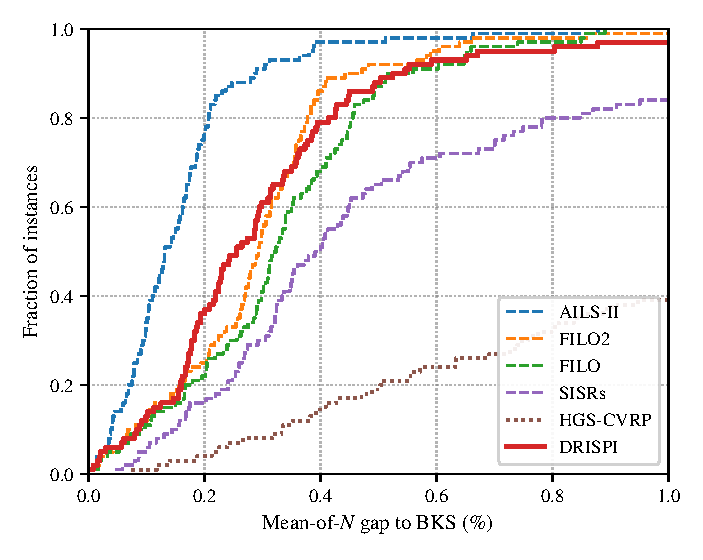
\includegraphics[width=0.8\textwidth]{figures/gap_ecdf.pdf}
\caption{Empirical CDF of the Mean-of-$N$ Gap to the Current BKS.} \label{fig:gap-ecdf}
\end{figure}

Figure~\ref{fig:gap-ecdf} shows why the Table~\ref{tab:solver-summary} means understate \gls{drispi}'s typical result and its tail at once: \gls{drispi}'s mean-of-3 gap has a mean of 0.309\% against a median of 0.255\% (interquartile range 0.172\%--0.380\%, ninetieth percentile 0.527\%, maximum 1.683\%), a right-skewed distribution in which most instances sit below the mean and a short tail sits well above it. \gls{drispi}'s curve tracks above FILO2's up to a gap of about 0.3\% (61\% of instances at or below that gap, against 55\% for FILO2) and falls below it from 0.4\% (79\% against 86\%), the crossover the non-significant paired mean-of-$N$ test against FILO2 allows: \gls{drispi} wins on the tighter half of the distribution and loses on the wider half. Against FILO, \gls{drispi}'s curve stays at or above FILO's over the range shown, consistent with the near-even 53-of-100 split in the paired test. HGS-CVRP's curve sits below all five other curves across the entire range shown: only 39\% of its instances reach a gap of one percent or less, and it does not visibly approach the other curves anywhere in the figure, consistent with the wide, significant margin the paired test above reports against it.

Table~\ref{tab:gap-tail} lists the instances behind that tail, the largest mean-of-3 gaps in Table~\ref{tab:xl-summary}, in descending order down to about $+0.6$ percent.

\begin{table}[H]
\centering
\caption{\gls{drispi}'s Largest Mean-of-3 Gap to Current \gls{bks} (Abbr. as per Section~\ref{sec:stu-dataset}).}
\label{tab:gap-tail}
\begin{tabular}{@{}lrlllrr@{}}
\toprule
Instance & $n$ & Depot & Customers & Demand & $r$ & Mean-of-3 Gap (\%) \\
\midrule
XL-n9571-k55 & 9{,}571 & R & R & Q & 174.7 & +1.68 \\
XL-n6034-k61 & 6{,}034 & R & C (5) & 5-10 & 98.9 & +1.18 \\
XL-n2634-k17 & 2{,}634 & R & C (4) & 1-10 & 162.6 & +1.17 \\
XL-n5174-k55 & 5{,}174 & C & C (6) & 1-10 & 94.1 & +0.88 \\
XL-n8207-k108 & 8{,}207 & C & C (2) & 1-10 & 75.9 & +0.80 \\
XL-n5902-k122 & 5{,}902 & E & RC (3) & Q & 48.8 & +0.67 \\
XL-n8028-k294 & 8{,}028 & C & R & Q & 27.3 & +0.65 \\
\bottomrule
\end{tabular}
\end{table}

Five of these seven instances fall in the dataset's ultra-long route band, $r \geq 50$ (Section~\ref{sec:stu-dataset}); Section~\ref{sec:stu-characteristics} takes up this concentration directly.

Two individual results do not appear in any aggregate. On XL-n4535-k1134, \gls{drispi}'s best-of-3 cost of 1,203,553 is below the initial \gls{bks} of 1,203,566 \citet{queirogaXLInstancesCapacitated2026} reported at publication. On XL-n1094-k157, \gls{drispi}'s best-of-3 cost matches both the initial and the current \gls{bks} exactly, at 112,431. Across all 100 instances, \gls{drispi}'s best-of-3 cost matches or beats AILS-II's mean-of-60 on 12 instances, listed in Table~\ref{tab:matches-beats}.

\begin{table}[H]
\centering
\caption{\gls{drispi}'s Best-of-3 Cost Matching or Beating a Published Reference.}
\label{tab:matches-beats}
\begin{tabular}{@{}lrrrl@{}}
\toprule
Instance & $r$ & \gls{drispi} Best-of-3 & Reference Cost & Reference \\
\midrule
XL-n1094-k157 & 7.8 & 112{,}431 & 112{,}431.0 & Initial \& current \gls{bks} \\
XL-n1281-k29 & 45.5 & 31{,}161 & 31{,}201.3 & AILS-II mean-of-60 \\
XL-n1328-k19 & 72.6 & 38{,}261 & 38{,}317.4 & AILS-II mean-of-60 \\
XL-n1374-k278 & 4.9 & 233{,}247 & 233{,}248.0 & AILS-II mean-of-60 \\
XL-n1654-k11 & 155.4 & 36{,}420 & 36{,}429.1 & AILS-II mean-of-60 \\
XL-n1794-k163 & 11.2 & 141{,}739 & 141{,}777.6 & AILS-II mean-of-60 \\
XL-n1981-k13 & 153.5 & 32{,}597 & 32{,}639.1 & AILS-II mean-of-60 \\
XL-n2307-k34 & 69.6 & 47{,}980 & 48{,}020.2 & AILS-II mean-of-60 \\
XL-n2727-k546 & 5.3 & 431{,}165 & 431{,}173.0 & AILS-II mean-of-60 \\
XL-n3804-k29 & 134.0 & 52{,}930 & 52{,}935.8 & AILS-II mean-of-60 \\
XL-n3888-k1010 & 4.2 & 1{,}881{,}512 & 1{,}882{,}369.0 & AILS-II mean-of-60 \\
XL-n4535-k1134 & 4.3 & 1{,}203{,}553 & 1{,}203{,}566.0 & Initial \gls{bks} \\
\bottomrule
\end{tabular}
\end{table}

\subsection{Performance by Instance Characteristics}\label{sec:stu-characteristics}
The XL instance set varies two candidate notions of scale at once: the customer count $n$ and the target average route length $r$ (Section~\ref{sec:stu-dataset}). The two are not interchangeable stand-ins for the same underlying quantity. $r$ is not derived from $n$; it is an independent design factor of the benchmark's own generation scheme, which fixes vehicle capacity $Q$ and fleet size jointly so that a minimum-route solution attains the target $r$ for whatever $n$ the instance happens to have, so the 100-instance design deliberately crosses a wide range of $r$ against a wide range of $n$ rather than letting one determine the other. For \gls{drispi} specifically, the two also act on the pipeline differently: $n$ sets how many customers decomposition has to distribute across $k$ subclusters, while $r$ sets how many stops a single vehicle round trip covers on average and, by construction, compresses the number of routes relative to customers once it grows large. A regression that treats $n$ as the only scale variable therefore risks crediting to instance size a pattern that a small number of long-route instances are actually driving.

A linear regression of the mean-of-3 gap on $n$ over all 100 instances gives a slope of \todo{NUMBER: gap-on-$n$ slope, all 100 instances} (test statistic \todo{NUMBER: gap-on-$n$ test statistic, all 100 instances}, $p = $~\todo{NUMBER: gap-on-$n$ p-value, all 100 instances}, 95\% confidence interval \todo{NUMBER: gap-on-$n$ 95\% CI, all 100 instances}). We define the long-route instances as those in the dataset's own ultra-long route band, $r \geq 50$ (Section~\ref{sec:stu-dataset}), a threshold fixed by the benchmark's band definition rather than chosen after inspecting the gaps, and it separates 14 long-route instances from the remaining 86. Restricting the same regression to those 86 instances changes the slope to \todo{NUMBER: gap-on-$n$ slope, $r<50$ only} (test statistic \todo{NUMBER: gap-on-$n$ test statistic, $r<50$ only}, $p = $~\todo{NUMBER: gap-on-$n$ p-value, $r<50$ only}, 95\% confidence interval \todo{NUMBER: gap-on-$n$ 95\% CI, $r<50$ only}). \todo{NUMBER: state here, once both p-values above are filled in, whether the $n$-slope loses significance on the $r<50$ subset}. If it does, the scale-gap relationship measured over all 100 instances is carried substantially by the 14 long-route instances rather than by instance size on its own.

This pattern is consistent with what decomposition does to a long route rather than with a direct effect of $n$. Every clustering method in Table~\ref{tab:decomp-methods} draws its partition from customer coordinates or route centroids and the dissimilarity metric of Equation~\ref{eq:decomp-dissimilarity}, without reference to which vehicle will eventually need which customers; a long route spans a customer set spread further apart on average than a short route serving a comparable number of stops, and that same spatial spread makes it more likely that some clustering cut line passes through the route rather than around it. Once a long route straddles a cluster boundary this way, the routing stage (Section~\ref{sec:fra-routing}) still solves each side of the cut to a good local optimum in isolation, but the seam between them is exactly the kind of defect BG-AILS exists to repair (Section~\ref{sec:fra-bg-ails}). BG-AILS repairs every seam in an instance under the same fixed chain length of $k$ cross-reconnects and the same wall-clock budget of Equation~\ref{eq:bg-ails-budget} regardless of how many of those seams cut through a long route rather than a short one, so an instance whose long routes cross more boundaries has more repair work competing for a budget that does not grow to match it.

Figure~\ref{fig:characteristics-panels} sets this account against the remaining instance characteristics descriptively: depot position, customer distribution, demand distribution, and $n$, each summarized by the per-category mean-of-3 gap (panels a-c) or plotted directly against the per-instance gap (panel d), rather than argued from.

\begin{figure}[H]
\centering
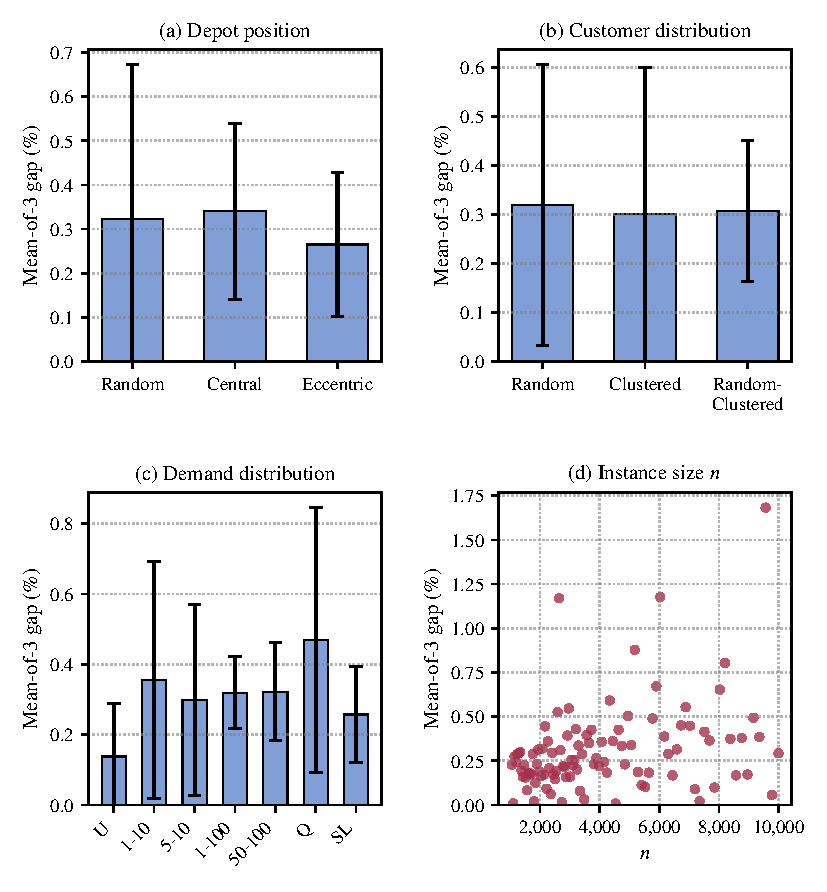
\includegraphics[width=0.85\textwidth]{figures/characteristics_panels.pdf}
\caption{Mean-of-3 Gap to the Current \gls{bks} by Instance Characteristic, Across All 100 XL instances (Error Bars Are One Sample Standard Deviation).}
\label{fig:characteristics-panels}
\end{figure}

\subsection{HAOS Weights}\label{sec:stu-haos}
Investigate how HAOS weights are converging and if there are obvious tendencies. Interpret the results. 

Are some HAOS levels converging always to the same result? Are some HAOS levels always converging in a similar way subject to the instance characteristics? Whats the variance in HAOS weight convergence? Do they differ a lot from seed to seed and are sensitive to randomness?

Are the results interpretable in general?

\subsection{Convergence Behavior}\label{sec:stu-convergence}
Show how the convergence behavior is like for \gls{drispi} by wallclock time and iterations. Use this chapter to also investigate improvement sources (quantitatively and qualitatively).